\documentclass{article}

\usepackage{graphicx}
\usepackage{tikz}
\usepackage{tikzsymbols}
\usetikzlibrary{calc,patterns,shapes.geometric}
\pagestyle{empty}
\usepackage[margin=0pt]{geometry}
\geometry{papersize={14in,12in}}

\def\centerarc[#1](#2)(#3:#4:#5){\draw[#1] ($(#2)+({#5*cos(#3)},{#5*sin(#3)})$) arc (#3:#4:#5);}

\begin{document}
	\begin{figure}
		\centering
		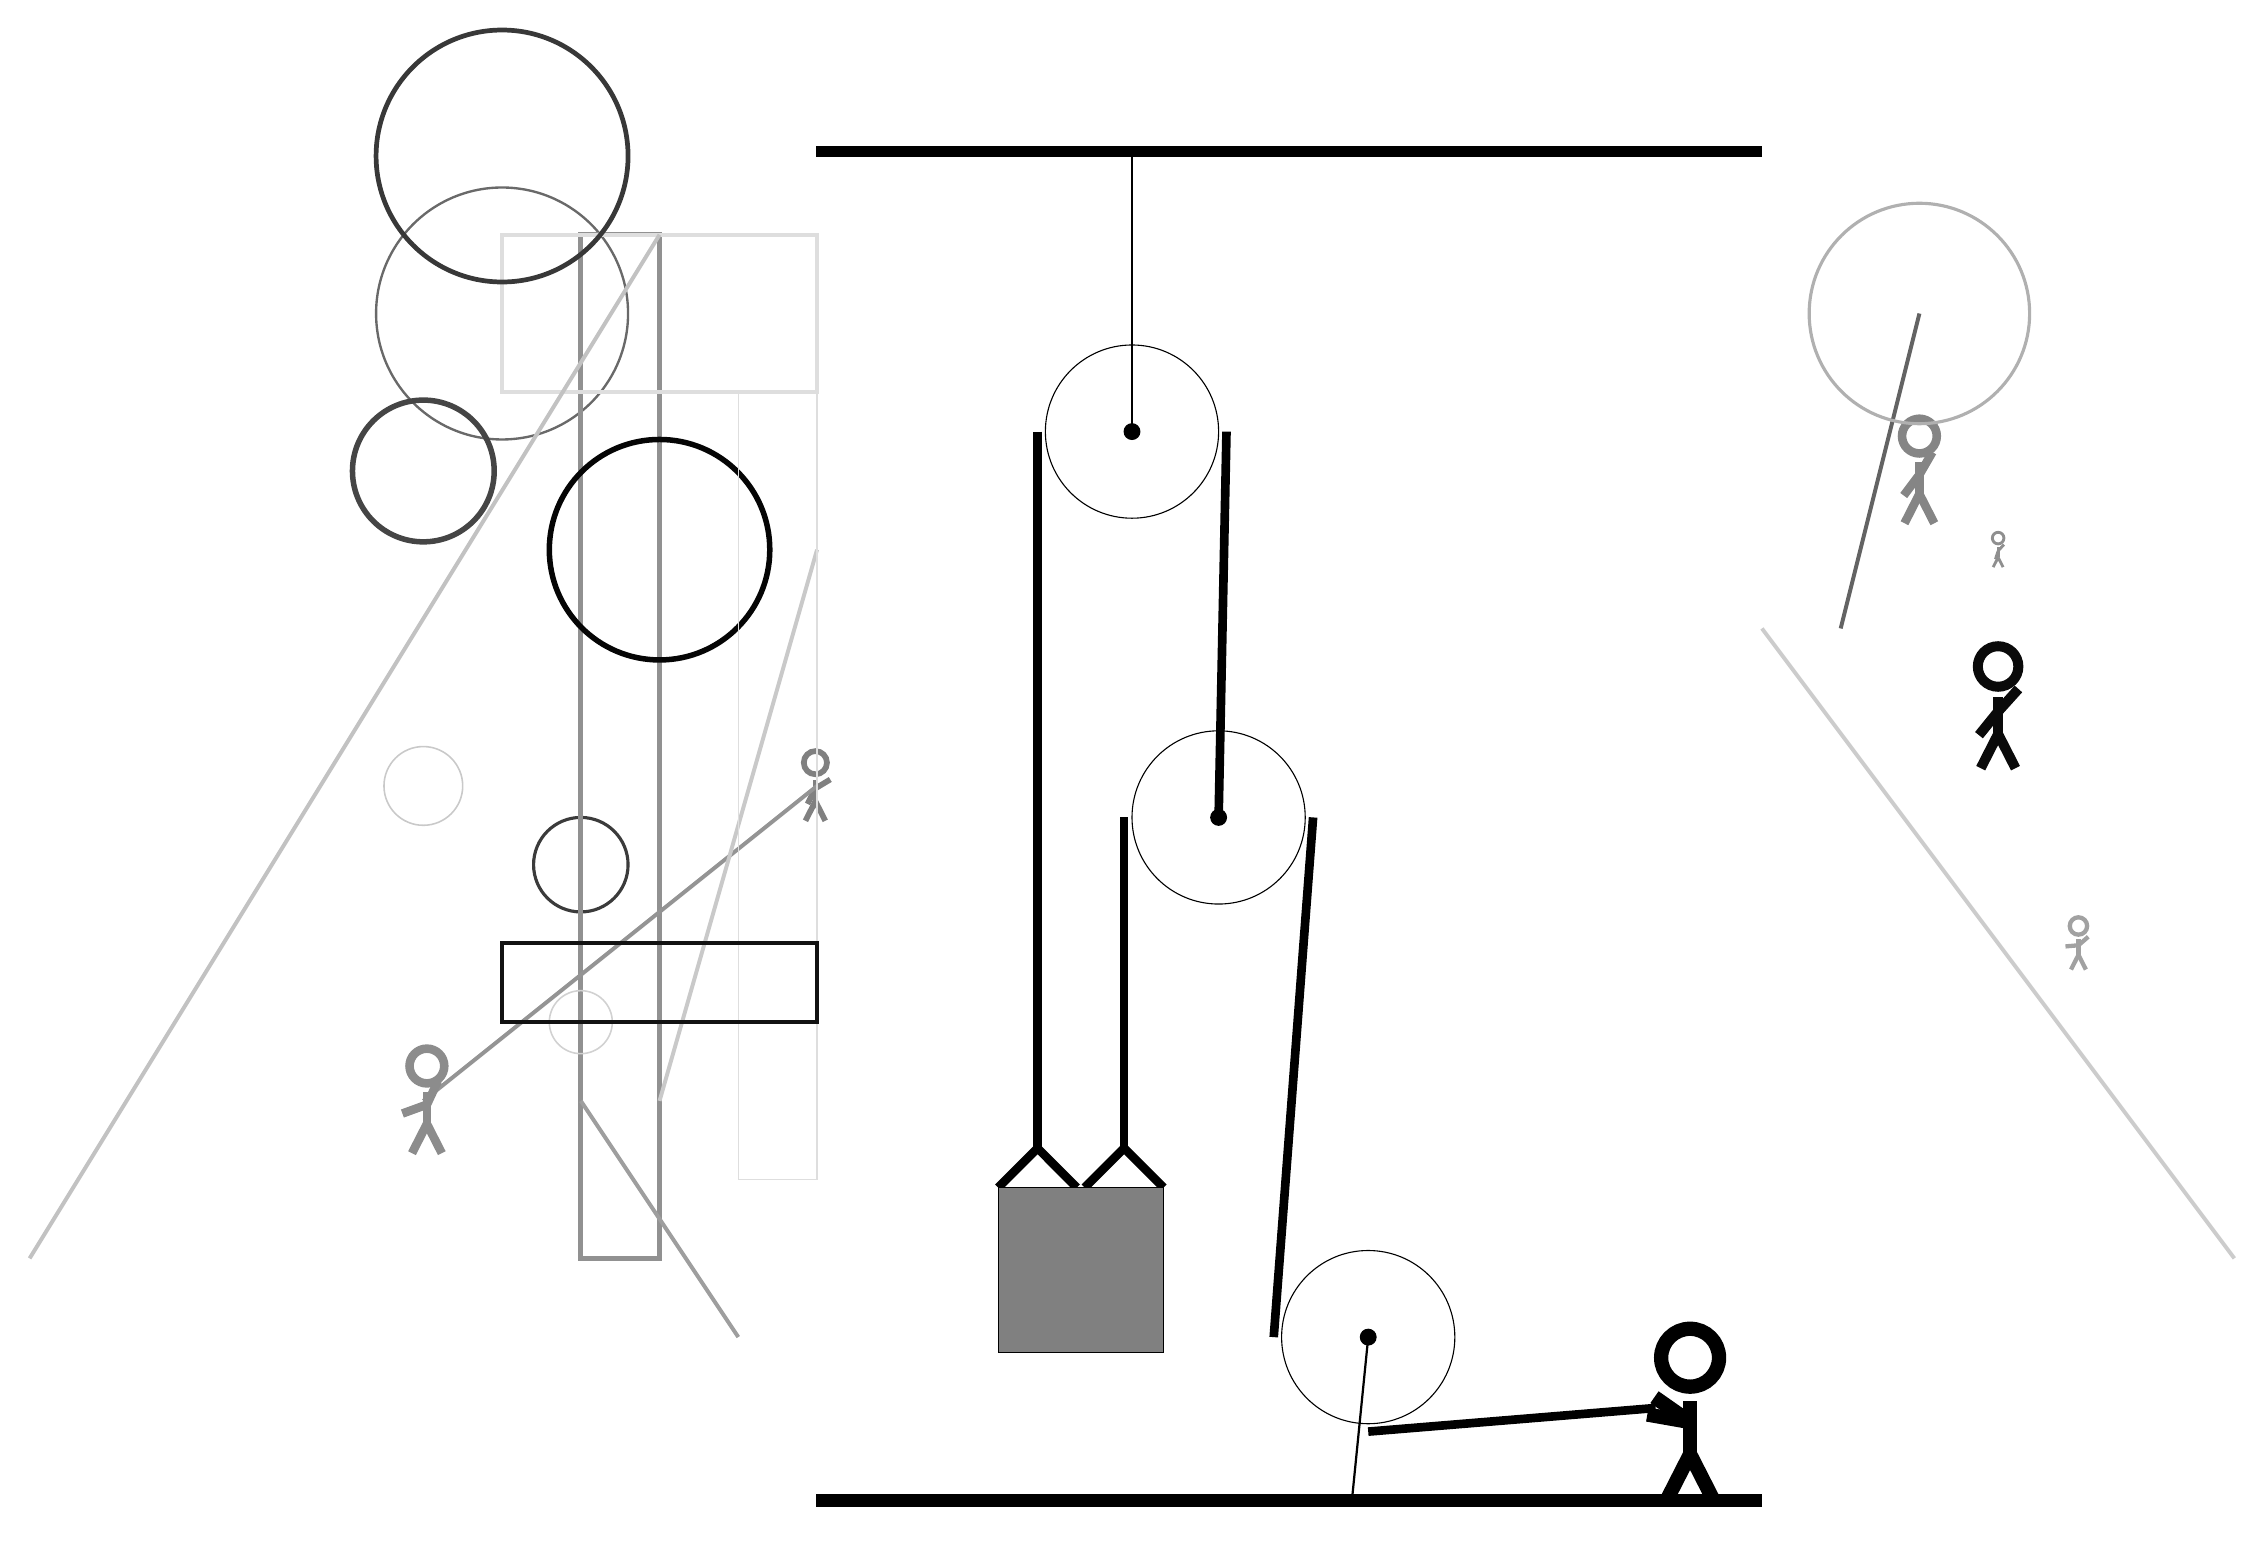
\begin{tikzpicture}
			%%%%% START %%%%%
			
			\draw[fill=black] (-2, 14) rectangle (10, 14.125);
			
			\draw (2, 10.5) circle (1.1);
			\draw[fill=black] (2, 10.5) circle (0.1);
			\draw[thick] (2, 10.5) -- (2, 14);
			
			\draw [line width=0.4mm, color=black!77](-5, 5) circle (0.6);
			
			\node[line width=0.7mm, color=black!50] at (-2, 6) {\Strichmaxerl[4][63][31]};
			\draw [line width=0.3mm, color=black!59](-6, 12) circle (1.6);
			\draw[line width=0.5mm, color=black!20](10, 8) -- (16, 0);
			\draw[line width=0.6mm, color=black!43] (-4, 0) rectangle (-5, 13);
			\node[line width=0.5mm, color=black!44] at (13, 9) {\Strichmaxerl[2][72][48]};
			\draw[line width=0.5mm, color=black!42](-2, 6) -- (-7, 2);
			
			\draw[line width=0.5mm, color=black!61](11, 8) -- (12, 12);
			\draw[line width=0.5mm, color=black!21](-2, 9) -- (-4, 2);
			\node[line width=0.6mm, color=black!45] at (-7, 2) {\Strichmaxerl[6][20][65]};
			\node[line width=0.2mm, color=black!96] at (13, 7) {\Strichmaxerl[7][51][48]};
			\draw [line width=0.7mm, color=black!73](-7, 10) circle (0.9);
			\draw[line width=0.5mm, color=black!13] (-2, 11) rectangle (-6, 13);
			
			\draw [line width=0.7mm, color=black!98](-4, 9) circle (1.4);
			\draw[line width=0.5mm, color=black!24](-4, 13) -- (-12, 0);
			\node[line width=0.5mm, color=black!48] at (12, 10) {\Strichmaxerl[6][53][60]};
			\draw[line width=0.2mm, color=black!13] (-2, 11) rectangle (-3, 1);
			\draw [line width=0.2mm, color=black!21](-7, 6) circle (0.5);
			\node[line width=0.5mm, color=black!37] at (14, 4) {\Strichmaxerl[3][5][41]};
			\draw [line width=0.4mm, color=black!31](12, 12) circle (1.4);
			\draw[line width=0.5mm, color=black!38](-3, -1) -- (-5, 2);
			
			\draw [line width=0.6mm, color=black!78](-6, 14) circle (1.6);
			
			\draw [line width=0.2mm, color=black!18](-5, 3) circle (0.4);
			\draw[line width=0.5mm, color=black!93] (-2, 4) rectangle (-6, 3);
			
			\draw (3.1, 5.6) circle (1.1);
			\draw[fill=black] (3.1, 5.6) circle (0.1);
			
			\draw (5, -1) circle (1.1);
			\draw[fill=black] (5, -1) circle (0.1);
			\draw[thick] (5, -1) -- (4.8, -3);
			
			\draw[line width = 1.1mm]  (0.3, 0.9) -- (0.8, 1.4) -- (1.3, 0.9);
			\draw[line width = 1.1mm]  (1.4, 0.9) -- (1.9, 1.4) -- (2.4, 0.9);
			\draw[fill=black!50] (0.3, 0.9) rectangle (2.4, -1.2);
			
			\draw[line width = 1.1mm] (0.8, 10.5) -- (0.8, 1.4);
			\centerarc[line width = 1.1mm](2, 10.5)(0:180:1.2000000000000002);
			\draw[line width = 1.1mm] (3.2, 10.5) -- (3.1, 5.6);
			\draw[line width = 1.1mm] (1.9, 5.6) -- (1.9, 1.4);
			\centerarc[line width = 1.1mm](3.1, 5.6)(0:180:1.2000000000000002);
			\draw[line width = 1.1mm] (4.3, 5.6) -- (3.8, -1);
			\centerarc[line width = 1.1mm](5, -1)(180:270:1.2000000000000002);
			\draw[line width = 1.1mm] (5, -2.2) -- (8.65, -1.9);
			
			\node at (9, -2) {\Strichmaxerl[10][-35][170]};
			
			\draw[fill=black] (-2, -3) rectangle (10, -3.15);
			
			%%%%% END %%%%%
		\end{tikzpicture}
	\end{figure}	
\end{document}